%% March 2018
%%%%%%%%%%%%%%%%%%%%%%%%%%%%%%%%%%%%%%%%%%%%%%%%%%%%%%%%%%%%%%%%%%%%%%%%%%%%
% AGUJournalTemplate.tex: this template file is for articles formatted with LaTeX
%
% This file includes commands and instructions
% given in the order necessary to produce a final output that will
% satisfy AGU requirements, including customized APA reference formatting.
%
% You may copy this file and give it your
% article name, and enter your text.
%
%%%%%%%%%%%%%%%%%%%%%%%%%%%%%%%%%%%%%%%%%%%%%%%%%%%%%%%%%%%%%%%%%%%%%%%%%%%%
% PLEASE DO NOT USE YOUR OWN MACROS
% DO NOT USE \newcommand, \renewcommand, or \def, etc.
%
% FOR FIGURES, DO NOT USE \psfrag or \subfigure.
% DO NOT USE \psfrag or \subfigure commands.
%%%%%%%%%%%%%%%%%%%%%%%%%%%%%%%%%%%%%%%%%%%%%%%%%%%%%%%%%%%%%%%%%%%%%%%%%%%%
%
% Step 1: Set the \documentclass
%
% There are two options for article format:
%
% PLEASE USE THE DRAFT OPTION TO SUBMIT YOUR PAPERS.
% The draft option produces double spaced output.
%

%% To submit your paper:
\documentclass[draft,linenumbers]{agujournal2018}
\usepackage{apacite}
\usepackage{url} %this package should fix any errors with URLs in refs.

%%%%%%%
% \usepackage{trackchanges}
% uncomment the line above to use the TrackChanges package to mark revisions if needed.
% The trackchanges package adds five new LaTeX commands:
%
%  \note[editor]{The note}
%  \annote[editor]{Text to annotate}{The note}
%  \add[editor]{Text to add}
%  \remove[editor]{Text to remove}
%  \change[editor]{Text to remove}{Text to add}
%
% complete documentation is here: http://trackchanges.sourceforge.net/
%%%%%%%

\draftfalse

% Now, type in the journal name: \journalname{<Journal Name>}

% ie, \journalname{Journal of Geophysical Research}
%% Choose from this list of Journals:
%
% JGR-Atmospheres
% JGR-Biogeosciences
% JGR-Earth Surface
% JGR-Oceans
% JGR-Planets
% JGR-Solid Earth
% JGR-Space Physics
% Global Biochemical Cycles
% Geophysical Research Letters
% Paleoceanography
% Radio Science
% Reviews of Geophysics
% Tectonics
% Space Weather
% Water Resource Research
% Geochemistry, Geophysics, Geosystems
% Journal of Advances in Modeling Earth Systems (JAMES)
% Earth's Future
% Earth and Space Science
% Geohealth
%

\journalname{Water Resource Research}

\usepackage{textgreek}

\begin{document}

%% ------------------------------------------------------------------------ %%
%  Title
%
% (A title should be specific, informative, and brief. Use
% abbreviations only if they are defined in the abstract. Titles that
% start with general keywords then specific terms are optimized in
% searches)
%
%% ------------------------------------------------------------------------ %%

% Example: \title{This is a test title}

\title{An Implementation of a Convolutional Neural Network for Fast segmentation of 4D microtomography volumes from fluid flow experiments in porous media.}

%% ------------------------------------------------------------------------ %%
%
%  AUTHORS AND AFFILIATIONS
%
%% ------------------------------------------------------------------------ %%

% Authors are individuals who have significantly contributed to the
% research and preparation of the article. Group authors are allowed, if
% each author in the group is separately identified in an appendix.)

% List authors by first name or initial followed by last name and
% separated by commas. Use \affil{} to number affiliations, and
% \thanks{} for author notes.
% Additional author notes should be indicated with \thanks{} (for
% example, for current addresses).

% Example: \authors{A. B. Author\affil{1}\thanks{Current address, Antartica}, B. C. Author\affil{2,3}, and D. E.
% Author\affil{3,4}\thanks{Also funded by Monsanto.}}

\authors{Y.Yang, I.B.Butler,F.Fusseis....}


% \affiliation{1}{First Affiliation}
% \affiliation{2}{Second Affiliation}
% \affiliation{3}{Third Affiliation}
% \affiliation{4}{Fourth Affiliation}

\affiliation{1}{University of Edinburgh}
%(repeat as many times as is necessary)

%% Corresponding Author:
% Corresponding author mailing address and e-mail address:

% (include name and email addresses of the corresponding author.  More
% than one corresponding author is allowed in this LaTeX file and for
% publication; but only one corresponding author is allowed in our
% editorial system.)

% Example: \correspondingauthor{First and Last Name}{email@address.edu}

\correspondingauthor{Yili YANG}{yili.yang@ed.ac.uk}

%% Keypoints, final entry on title page.

% Example:
% \begin{keypoints}
% \item	List up to three key points (at least one is required)
% \item	Key Points summarize the main points and conclusions of the article
% \item	Each must be 100 characters or less with no special characters or punctuation
% \end{keypoints}

%  List up to three key points (at least one is required)
%  Key Points summarize the main points and conclusions of the article
%  Each must be 100 characters or less with no special characters or punctuation

\begin{keypoints}
\item An effective solution to the segmentation of extremely large and compromised quality synchrotron CT data set using convolutional neuron network.

\end{keypoints}

%% ------------------------------------------------------------------------ %%
%
%  ABSTRACT
%
% A good abstract will begin with a short description of the problem
% being addressed, briefly describe the new data or analyses, then
% briefly states the main conclusion(s) and how they are supported and
% uncertainties.
%% ------------------------------------------------------------------------ %%

%% \begin{abstract} starts the second page

\begin{abstract}
multiphase fluid flow in porous media is extensively studied for its application in enhanced
oil recovery and agriculture etc. We conducted two-phase flow experiments in carbonate rocks and
imaged real-time fluid displacement using high temporal-spatial resolution synchrotron micro-tomography. One side-effect of fast synchrotron CT imaging is compromised image quality,
such as more artifacts and poorer contrast, which make the images hard to be segmented. We implemented a convolutional neuron network and trained it with 14k+ images from multiphase flow experiments generated by synchrotron CT. The trained neuron network can segment highly noised synchrotron CT images of core-flooding experiments fast and accurately without any pre-processing of the raw image. Segmenting one CT volume of size 1003x496x496 takes about 10 minutes on a Nvidia Quadro K5200 GPU. On the test dataset, the interception over union reached 0.985 and mean accuracy of the three segmentation class reached 0.990.
\end{abstract}


%% ------------------------------------------------------------------------ %%
%
%  TEXT
%
%% ------------------------------------------------------------------------ %%

%%% Suggested section heads:
% \section{Introduction}
%
% The main text should start with an introduction. Except for short
% manuscripts (such as comments and replies), the text should be divided
% into sections, each with its own heading.

% Headings should be sentence fragments and do not begin with a
% lowercase letter or number. Examples of good headings are:

% \section{Materials and Methods}
% Here is text on Materials and Methods.
%
% \subsection{A descriptive heading about methods}
% More about Methods.
%
% \section{Data} (Or section title might be a descriptive heading about data)
%
% \section{Results} (Or section title might be a descriptive heading about the
% results)
%
% \section{Conclusions}


\section{Introduction}
\subsection{Multiphase fluid flow}
Multiphase flow in porous media is a universal yet complex phenomenon that related to many applications from hydrocarbon recovery to contaminant transport. Experimental studies of multiphase flow in porous media range from 2-D micro model experiments (e.g. \citet{keller1997micromodel}), to 3-D quasi-static core-flooding experiments (e.g. \citet{ott2012core}), to 4-D time resolved core-flooding experiment (e.g.\citet{pak2015droplet}; \citet{berg2014multiphase}). With experimental dimension increasing and the amount of collected data increasing exponentially, the observation is more approaching to reality. A 4-D time resolved CT data set is usually a few tera-bytes large. The efficiency of large-scale data processing is becoming the bottle-neck to these studies.

\subsection{Synchrotron CT imaging}
X-ray computed micro tomography (X-ray \textmu CT) is a non-destructive imaging technique that has spatial resolution for few microns, the duration of a single scan usually cost tens of minutes to an hour. It is impossible to capture important fluid behaviours such as snap-off with such speed. X-ray generated by synchrotron radiation has very high photon flux so that the image can be acquired in few seconds time scale (e.g. \citet{berg2014multiphase}), however the quality of the image has to be compromised for capturing short time fluid events. The degradation of image quality, usually means more noise, artifacts and poorer contrast, makes image segmentation difficult and time consuming.

\subsection{Deep learning image segmentation}
\subsubsection{Image segmentation}
Image segmentation is the classification of pixels in digital images into meaningful groups, for instance labelling kidney in a medical CT image. Image segmentation is the foundation of all consequential scientific analyses and conclusions. In this study we segment CT images taken from core-flooding experiments into three phases: solid, oil and water. The conventional segmentation methods mainly base on properties of similarity and discontinuity (\citet{gonzalez2002digital}): based on similarity, thresholding, region-growing (e.g. watershed (\citet{vincent1991watersheds}), and clustering (e.g. K-means (\citet{hartigan1979algorithm})) are catagories of region-based algorithms that resolve segmentation by partition images into similar regions. Based on discontinuity, edge-based algorithms attempt to segment image by locating the edges of different objects. These classical algorithms are usually used when the data quality is optimum, to produce efficient and accurate segmentation. Synchrotron \textmu CT compromise image quality to maximize temporal resolution, and a single synchrotron \textmu CT experiment usually produces few terabytes of data. When segmenting synchrotron \textmu CT images, it's usually becoming too time-taking to find the best combination of filterings, register images with masks, and tweak the parameter of each processing step to make the images segment-able using conventional algorithms. Besides the testing of workflows combinations, the pre-processing itself is extremely time-consuming, and no processing workflow can work as 'panacea' to a series of \textmu CT data sets, these problems are difficult to be tackled with conventional segmentation algorithms.

\subsubsection{Segmentation using convolutional neuron network}
Unlike conventional segmentation methods that only take a certain feature into account, deep learning allows models to abstract multiple levels of features to represent data. Convolutional neuron networks (CNNs, \citet{lecun1989backpropagation}) are a class of deep neuron network that have been proved effective in visual recognition tasks (e.g. \citet{krizhevsky2012imagenet}; \citet{long2015fully};\citet{girshick2014rich}). \citet{ronneberger2015u} also proved the reliability of CNN in segmenting low-contrast gray scale biomedical images which are similar to our data set. We used the CNN architecture 'U-Net' introduced by \citet{ronneberger2015u}, to train our data set and yield precise segmentation.


The training of a CNN model is a form of supervised learning. During training, the model is shown an image and output a prediction of probability that each pixel belongs to a category. Then the prediction is provided with a ground truth image to compare and measure the difference between output and target. The comparison is calculated by a criterion called loss function and yield a loss score. The model iteratively updates the internal adjustable parameters (neuron weights), as the training proceeds, to minimize the loss therefore improve the prediction step-wisely.


Loss is a measurement of how well a model is fit into the training data set, however it does not imply if the model is generalized enough to represent data beyond the training set (over-fit). Validation is a syn-training process that separate a small portion of the training data to monitor over-fit and tune hyper-parameters that control model's learning behaviour. During validation, the update of the neuron weights are prevented so the model stays unchanged, therefore validation can always represent the current model performance without bringing change to the model. Training loss keeps decreasing during training regardless of over-fit, because the model always tries to minimize the loss to fit better into the training data. However the validation loss can increase while the model is over-fitting and therefore can not represent validation data set any more. When training loss is significantly smaller than validation loss, model is under-fit, and when training loss is significantly larger than validation loss, model is over-fit, the best model is identified when training loss approaches validation loss. Criterion such as F1-score, Intersection over union (IoU) is often used to evaluate segmentation reliability during validation. Unlike loss function that measures the learning process, these criteria directly measure segmentation quality. Thus can be used as ultimate evaluation of the segmentation reliability. Similarly, when the model is over-fit, these measurements start dropping. When the validation loss is about to increase or the validation accuracy is about to decrease, training should be ceased, this technique is called early-stopping. 


When training is completed, a held-out test set is revealed to the CNN model to test its performance on entirely unfamiliar data. This set is absolutely 'unseen' by the CNN model so the test score can provide an unbiased evaluation of the reliability of the model prediction on real-world data.

\section{Materials and methods}
\subsection{multiphase fluid flow experiments}
A benchmark carbonate rock, Indiana limestone, was used as porous medium in the experiments.The rock was cored and installed in an X-ray transparent cell designed by \citet{fusseis2014low}. For fluid injection we used mineral oil and Potassium Iodine solution as oil and aqueous phase respectively. Synchrotron X-ray Images were acquired using pink beam by one second acquisition time in every 20 seconds during fluid injections. We used the beam line 2-BM at the Advanced Photon Source in Argonne National Laboratory in Chicago, U.S.

\subsection{Convolutional neuron network segmentation}
\subsubsection{Data preparation}
The raw CT projections were reconstructed using Octopus8\texttrademark. We segmented all the reconstructed images for ground-truthing. The original reconstructed images are hard to be segmented due to noises, artifacts and low contrast between solid and brine. With a high-resolution reference dry scan (before fluid injection) available, we segmented the solid phase and use it as mask in wet scans to further separate the three phases. We used Non-local Means (implemented in Fiji-ImageJ) filter to denoise the reconstructed images, registered and applied the mask using Avizo9\texttrademark, and implemented the seeded random-walker (Scikit-image) algorithm to finalize the segmentation. The whole segmentation work flow is very time-consuming and uses different softwares thus difficult to automate.

Every original reconstruction image was paired with the corresponding segmented image to make a pair of input-target image set for the network training. A total of 18 CT volumes were divided into 14 training sets, 2 test sets and 2 validation set. Each CT volume had 1003 reconstruction images of size 496x496.  
 \
 \begin{figure}[h]
 \centering
 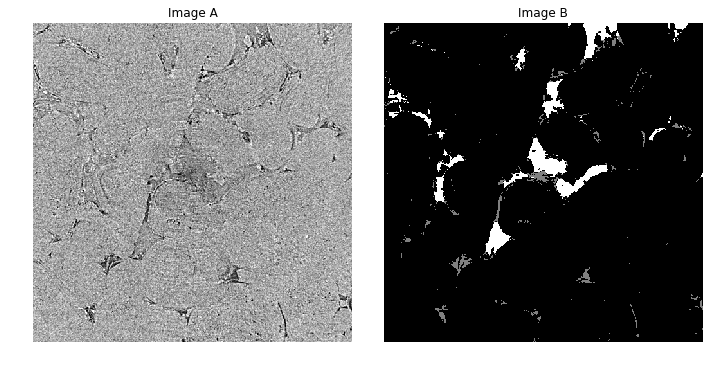
\includegraphics[width=33pc]{imgs/17_test_original.png}
 \caption{Image A shows the input image that is raw reconstruction image. Image B shows the corresponding ground truth image segmented by seeded random walker algorithm}
 \label{fig1}
 \end{figure}
 
\subsubsection{Network training}
We used the CNN architecture U-net introduced by \citet{ronneberger2015u} and implemented by Joris \citet{Jorispytorch} using the open-sourced deep learning platform Pytorch (\citet{paszke2017automatic}). 

The CNN training was set to 50 Epochs, at learning rate of 5e-5. Each epoch is a full iteration of all training sets. Loss of input and output was calculated for every image and back-propagated to update the neuron weights in order to  minimize the loss therefore improving the prediction. Pytorch built-in cross entropy loss function was used as the loss function during training. Cross entropy loss function calculates the distance between the two probability distributions - the output and the corresponding ground-truth. The loss value was step-wisely reduced and finally converged at the end of training. 

%\begin{equation}
%{loss}(x, class) = -\log\left(\frac{\exp(x[class])}{\sum_j\exp(x[j])}\right)
%                       = -x[class] + \log\left(\sum_j \exp(x[j])\right)
%\end{equation}

The sequence of the input data was shuffled at the start of each epoch so that the neuron weights updated in each iteration were different. The optimizer used was Pytorch built-in Adam algorithm (\citet{kingma2014adam}). L2 regularization 1e-5 was applied to alleviate over-fitting.

We used a NVidia\texttrademark Quadro K5200 GPU (8GB) to train the network. Batch size is one of the important hyper-parameters that partition the training set into mini-batches. In this study batch size was 1 because of limited GPU memory.

\subsubsection{Validation}
We used intersection over union (IoU) and accuracy as the metric of segmentation accuracy. IoU is the ratio of intersection - the overlapping area between prediction and ground truth - and union - the area encompassed by both prediction and ground truth (eq.1). Accuracy is another evaluation metric of binary classification, it is the ratio of correctly classified pixels and total pixels. First we take probability above 95\% in prediction as true, then calculate the true positive (TP), false positive (FP), true negative (TN) and false negative (FN) w.r.t. the ground truth. The accuracy was calculated using eq.2:

\begin{equation}
    IoU=\frac{Area-of-Overlap}{Area-of-Union}
\end{equation}
\begin{equation}
    accuracy=\frac{TP+TN}{TP+TN+FP+FN}
\end{equation}

Loss, accuracy and IoU of the validation set was calculated after every training epoch. When the accuracy or IoU of the validation set stopped increasing or the validation loss started to increasing, the model was over-fit and training should be stopped. In practice the early-stopping point was the 28th epoch (Fig.2), the criterion for early-stopping is validation loss increasing for consecutively five epochs.

\begin{figure}[h]
 \centering
 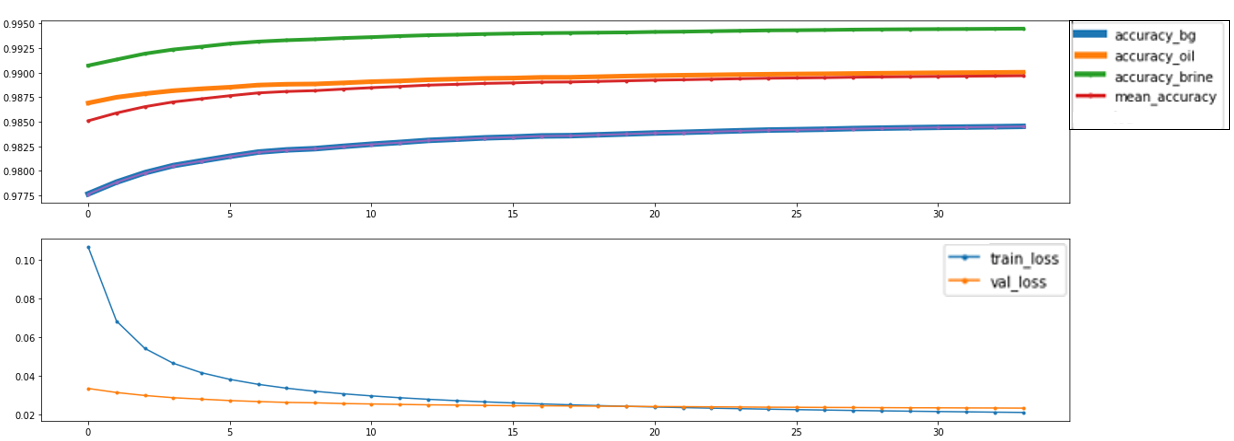
\includegraphics[width=33pc]{imgs/training_result_23oct.png}
 \caption{Upper Image shows phase accuracy and IoU improvement during validation. Lower image shows training loss and validation loss comparison during training.}
 \label{fig2}
 \end{figure}

\subsubsection{Testing}
After training, it's necessary to test the performance of the CNN model on 'unseen' data to check its generalization and visually assess the segmentation quality on real-world data. The well-separated test data sets were first-time input into the trained neuron network model. IOU and individual phase accuracy were calculated as the measurements of model accuracy. The output images were visualized as final segmentation result of real-world data.


Fig.2 upper image shows the syn-training validation accuracy and IoU was steadily increasing. And lower image shows that the model was under-fit in the beginning, and training loss rapidly decreased and overtook the validation loss at the 17th epoch, which was identified as the best-fit. 

\section{Results}
\subsection{Testing Result of the trained network}

The total training time was 148 hours, the complete training set was trained for 24 epochs and the best fit was identified at the 17th epoch (Fig.2). The testing took 10 minutes for the test data set sized 2006x496x496.

The accuracy measured on the test set shows high accuracy and IoU of all catagories. The segmentation accuracy of background (solid) reached 98.51\%, oil phase accuracy reached 99.13\%, brine phase accuracy reached 99.37\% and on average 99.00\%.
The average IoU of the test set measured is 98.51\%.

%'accuracy bg': 0.9850739795759733, 'accuracy oil': 0.9913017998246347, 'accuracy brine': 0.9937333781419594, 'mean accuracy': 0.9900363858475222, 'iou': 0.9850545787712824 finished

\begin{figure}[h]
 \centering
 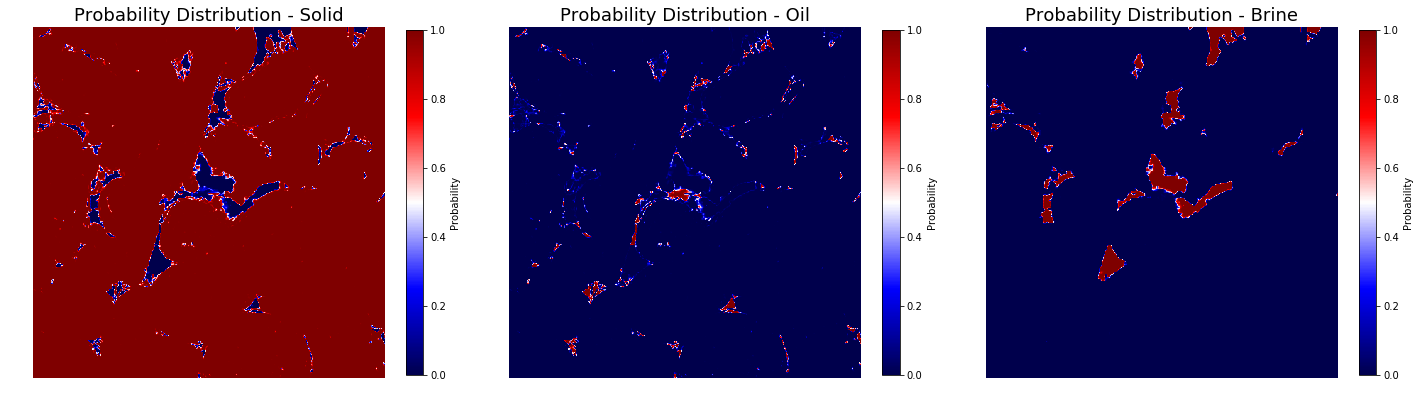
\includegraphics[width=33pc]{imgs/17_test_probmap.png}
 \caption{Probability distribution of phase segmentation}
 \label{fig3}
 \end{figure}
 
The probability (Fig.3) distribution map is generated by the Pytorch built-in softmax function that transforms the model output to a probability distribution output into 0-1 distribution. It visualised the probability distribution of all three phases. The colour map indicates the likely-hood of a pixel belonging to one phase. The red end is extremely likely, the blue end is extremely unlikely, and white is ambiguous likely-hood. The three phases are easily determined because the ambiguous likely-hood pixels are of minor amounts. It also illustrates a very robust determination of the model in segmentation. 

\begin{figure}[h]
 \centering
 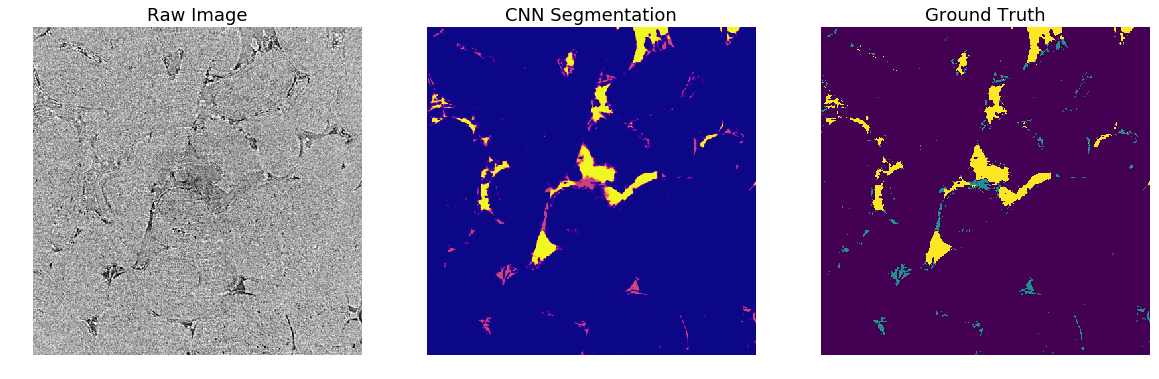
\includegraphics[width=33pc]{imgs/17_test_result.png}
 \caption{Comparison of input raw image, CNN segmentation result and ground truth}
 \label{fig4}
 \end{figure}

Take probability above 95\% as foreground and below 94\% as background for each phase, the segmentation result is shown in Fig.4. The visualization (Fig.4) of CNN segmentation shows high similarity with ground truth. Minor differences are existed but hardly recognized visually. The result proves that the trained network is reliable in segmenting highly noised, low contrast CT reconstructed images.

\section{Discussion}
\subsection{Future improvements}
Comparison of different network architectures can be further tested. Apart from the U-net, there are other powerful CNN architectures such as ResNet (\citet{he2016deep}), GoogLeNet (\citet{szegedy2015going}), VGGNet (\citet{simonyan2014very}) etc. with different advantages and specialities. It still remains to be tested on which is the most suitable architecture for segmenting \textmu CT images from multiphase fluid flow experiments.

Different hyper-parameters such as learning rate, batch size, normalisation index, network depth etc. can be further tested to find the optimal training efficiency and result.

The current training data set can be augmented by noising, flipping, rotating, scaling, cropping or translating the original training images. Data augmentation allows amplification of the training data set based on currently existed data set and therefore further generalize the CNN model for more robust segmentation of different data sets.

\subsection{Transfer learning}
By using future data sets of similar context, this model can be further trained. The imaging condition and materials can be different due to different rock types and different fluids used. The model will be increasingly robust and generalized as more data sets are fed. So the future training needed to classify future data will be decreased and converged to a point where no more training is needed. That becomes the ultimate model that can segment multiphase fluid flow experiment data regardless of noise, rocktype, fluid type and beamline condition etc.

\section{Conclusion}
The CNN segmentation can significantly improve the segmentation workflow for multiphase flow \textmu CT images. The advantages are fivefold. Firstly once a network for segmenting multiphase flow images is trained, it can be applied to future data without re-train. Second, once a network is trained it can function without a high quality reference image at time zero, allowing segmentation of any data set that lacks such a reference. Thirdly the segmentation is the direct output from reconstruction image, and so the considerable time consumed by preprocessing (tuning of filtering, registration, masking etc.) is no longer required. This is significant because for fast synchrotron \textmu CT data set, the data processing time is considerably long compared with time used for interpretation.Fourthly, the algorithm is capable for highly noised images, which is extremely limiting for conventional processing paths. Finally, the performance of the CNN network improves as more data it has seen, it evolves itself when it is used. Overall the CNN segmentation is a powerful and efficient tool for \textmu CT image segmentation, especially for extra-large and noisy data set.

%Text here ===>>>

%%

%  Numbered lines in equations:
%  To add line numbers to lines in equations,
%  \begin{linenomath*}
%  \begin{equation}
%  \end{equation}
%  \end{linenomath*}



%% Enter Figures and Tables near as possible to where they are first mentioned:
%
% DO NOT USE \psfrag or \subfigure commands.
%
% Figure captions go below the figure.
% Table titles go above tables;  other caption information
%  should be placed in last line of the table, using
% \multicolumn2l{$^a$ This is a table note.}
%
%----------------
% EXAMPLE FIGURE
%
% \begin{figure}[h]
% \centering
% when using pdflatex, use pdf file:
% \includegraphics[width=20pc]{figsamp.pdf}
%
% when using dvips, use .eps file:
% \includegraphics[width=20pc]{figsamp.eps}
%
% \caption{Short caption}
% \label{figone}
%  \end{figure}
%
% ---------------
% EXAMPLE TABLE
%
% \begin{table}
% \caption{Time of the Transition Between Phase 1 and Phase 2$^{a}$}
% \centering
% \begin{tabular}{l c}
% \hline
%  Run  & Time (min)  \\
% \hline
%   $l1$  & 260   \\
%   $l2$  & 300   \\
%   $l3$  & 340   \\
%   $h1$  & 270   \\
%   $h2$  & 250   \\
%   $h3$  & 380   \\
%   $r1$  & 370   \\
%   $r2$  & 390   \\
% \hline
% \multicolumn{2}{l}{$^{a}$Footnote text here.}
% \end{tabular}
% \end{table}

%% SIDEWAYS FIGURE and TABLE
% AGU prefers the use of {sidewaystable} over {landscapetable} as it causes fewer problems.
%
% \begin{sidewaysfigure}
% \includegraphics[width=20pc]{figsamp}
% \caption{caption here}
% \label{newfig}
% \end{sidewaysfigure}
%
%  \begin{sidewaystable}
%  \caption{Caption here}
% \label{tab:signif_gap_clos}
%  \begin{tabular}{ccc}
% one&two&three\\
% four&five&six
%  \end{tabular}
%  \end{sidewaystable}

%% If using numbered lines, please surround equations with \begin{linenomath*}...\end{linenomath*}
%\begin{linenomath*}
%\begin{equation}
%y|{f} \sim g(m, \sigma),
%\end{equation}
%\end{linenomath*}

%%% End of body of article

%%%%%%%%%%%%%%%%%%%%%%%%%%%%%%%%
%% Optional Appendix goes here
%
% The \appendix command resets counters and redefines section heads
%
% After typing \appendix
%
%\section{Here Is Appendix Title}
% will show
% A: Here Is Appendix Title
%
%appendix
%\section{Jupyter Notebook}

%%%%%%%%%%%%%%%%%%%%%%%%%%%%%%%%%%%%%%%%%%%%%%%%%%%%%%%%%%%%%%%%
%
% Optional Glossary, Notation or Acronym section goes here:
%
%%%%%%%%%%%%%%
% Glossary is only allowed in Reviews of Geophysics
%  \begin{glossary}
%  \term{Term}
%   Term Definition here
%  \term{Term}
%   Term Definition here
%  \term{Term}
%   Term Definition here
%  \end{glossary}

%
%%%%%%%%%%%%%%
% Acronyms
%   \begin{acronyms}
%   \acro{Acronym}
%   Definition here
%   \acro{EMOS}
%   Ensemble model output statistics
%   \acro{ECMWF}
%   Centre for Medium-Range Weather Forecasts
%   \end{acronyms}

%
%%%%%%%%%%%%%%
% Notation
%   \begin{notation}
%   \notation{$a+b$} Notation Definition here
%   \notation{$e=mc^2$}
%   Equation in German-born physicist Albert Einstein's theory of special
%  relativity that showed that the increased relativistic mass ($m$) of a
%  body comes from the energy of motion of the body—that is, its kinetic
%  energy ($E$)—divided by the speed of light squared ($c^2$).
%   \end{notation}




%%%%%%%%%%%%%%%%%%%%%%%%%%%%%%%%%%%%%%%%%%%%%%%%%%%%%%%%%%%%%%%%
%
%  ACKNOWLEDGMENTS
%
% The acknowledgments must list:
%
% >>>>	A statement that indicates to the reader where the data
% 	supporting the conclusions can be obtained (for example, in the
% 	references, tables, supporting information, and other databases).
%
% 	All funding sources related to this work from all authors
%
% 	Any real or perceived financial conflicts of interests for any
%	author
%
% 	Other affiliations for any author that may be perceived as
% 	having a conflict of interest with respect to the results of this
% 	paper.
%
%
% It is also the appropriate place to thank colleagues and other contributors.
% AGU does not normally allow dedications.


\acknowledgments
 This study is funded by Petrobras and Royal Dutch Shell via International Centre for Carbonate Reservoirs. 


%% ------------------------------------------------------------------------ %%
%% References and Citations

%%%%%%%%%%%%%%%%%%%%%%%%%%%%%%%%%%%%%%%%%%%%%%%
% BibTeX is preferred:
%
\bibliography{aguref.bib}
%
% no need to specify bibliographystyle
%%%%%%%%%%%%%%%%%%%%%%%%%%%%%%%%%%%%%%%%%%%%%%%


% Please use ONLY \citet and \citep for reference citations.
% DO NOT use other cite commands (e.g., \cite, \citeyear, \nocite, \citealp, etc.).
%% Example \citet and \citep:
%  ...as shown by \citet{Boug10}, \citet{Buiz07}, \citet{Fra10},
%  \citet{Ghel00}, and \citet{Leit74}.

%  ...as shown by \citep{Boug10}, \citep{Buiz07}, \citep{Fra10},
%  \citep{Ghel00, Leit74}.

%  ...has been shown \citep [e.g.,][]{Boug10,Buiz07,Fra10}.


\end{document}



More Information and Advice:

%% ------------------------------------------------------------------------ %%
%
%  SECTION HEADS
%
%% ------------------------------------------------------------------------ %%

% Capitalize the first letter of each word (except for
% prepositions, conjunctions, and articles that are
% three or fewer letters).

% AGU follows standard outline style; therefore, there cannot be a section 1 without
% a section 2, or a section 2.3.1 without a section 2.3.2.
% Please make sure your section numbers are balanced.
% ---------------
% Level 1 head
%
% Use the \section{} command to identify level 1 heads;
% type the appropriate head wording between the curly
% brackets, as shown below.
%
%An example:
%\section{Level 1 Head: Introduction}
%
% ---------------
% Level 2 head
%
% Use the \subsection{} command to identify level 2 heads.
%An example:
%\subsection{Level 2 Head}
%
% ---------------
% Level 3 head
%
% Use the \subsubsection{} command to identify level 3 heads
%An example:
%\subsubsection{Level 3 Head}
%
%---------------
% Level 4 head
%
% Use the \subsubsubsection{} command to identify level 3 heads
% An example:
%\subsubsubsection{Level 4 Head} An example.
%
%% ------------------------------------------------------------------------ %%
%
%  IN-TEXT LISTS
%
%% ------------------------------------------------------------------------ %%
%
% Do not use bulleted lists; enumerated lists are okay.
% \begin{enumerate}
% \item
% \item
% \item
% \end{enumerate}
%
%% ------------------------------------------------------------------------ %%
%
%  EQUATIONS
%
%% ------------------------------------------------------------------------ %%

% Single-line equations are centered.
% Equation arrays will appear left-aligned.

Math coded inside display math mode \[ ...\]
 will not be numbered, e.g.,:
 \[ x^2=y^2 + z^2\]

 Math coded inside \begin{equation} and \end{equation} will
 be automatically numbered, e.g.,:
 \begin{equation}
 x^2=y^2 + z^2
 \end{equation}


% To create multiline equations, use the
% \begin{eqnarray} and \end{eqnarray} environment
% as demonstrated below.
\begin{eqnarray}
  x_{1} & = & (x - x_{0}) \cos \Theta \nonumber \\
        && + (y - y_{0}) \sin \Theta  \nonumber \\
  y_{1} & = & -(x - x_{0}) \sin \Theta \nonumber \\
        && + (y - y_{0}) \cos \Theta.
\end{eqnarray}

%If you don't want an equation number, use the star form:
%\begin{eqnarray*}...\end{eqnarray*}

% Break each line at a sign of operation
% (+, -, etc.) if possible, with the sign of operation
% on the new line.

% Indent second and subsequent lines to align with
% the first character following the equal sign on the
% first line.

% Use an \hspace{} command to insert horizontal space
% into your equation if necessary. Place an appropriate
% unit of measure between the curly braces, e.g.
% \hspace{1in}; you may have to experiment to achieve
% the correct amount of space.


%% ------------------------------------------------------------------------ %%
%
%  EQUATION NUMBERING: COUNTER
%
%% ------------------------------------------------------------------------ %%

% You may change equation numbering by resetting
% the equation counter or by explicitly numbering
% an equation.

% To explicitly number an equation, type \eqnum{}
% (with the desired number between the brackets)
% after the \begin{equation} or \begin{eqnarray}
% command.  The \eqnum{} command will affect only
% the equation it appears with; LaTeX will number
% any equations appearing later in the manuscript
% according to the equation counter.
%

% If you have a multiline equation that needs only
% one equation number, use a \nonumber command in
% front of the double backslashes (\\) as shown in
% the multiline equation above.

% If you are using line numbers, remember to surround
% equations with \begin{linenomath*}...\end{linenomath*}

%  To add line numbers to lines in equations:
%  \begin{linenomath*}
%  \begin{equation}
%  \end{equation}
%  \end{linenomath*}



